% THIS IS SIGPROC-SP.TEX - VERSION 3.1


% WORKS WITH V3.2SP OF ACM_PROC_ARTICLE-SP.CLS
% APRIL 2009
%
% It is an example file showing how to use the 'acm_proc_article-sp.cls' V3.2SP
% LaTeX2e document class file for Conference Proceedings submissions.
% ----------------------------------------------------------------------------------------------------------------
% This .tex file (and associated .cls V3.2SP) *DOES NOT* produce:
%       1) The Permission Statement
%       2) The Conference (location) Info information
%       3) The Copyright Line with ACM data
%       4) Page numbering
% ---------------------------------------------------------------------------------------------------------------
% It is an example which *does* use the .bib file (from which the .bbl file
% is produced).
% REMEMBER HOWEVER: After having produced the .bbl file,
% and prior to final submission,
% you need to 'insert'  your .bbl file into your source .tex file so as to provide
% ONE 'self-contained' source file.
%
% Questions regarding SIGS should be sent to
% Adrienne Griscti ---> griscti@acm.org
%
% Questions/suggestions regarding the guidelines, .tex and .cls files, etc. to
% Gerald Murray ---> murray@hq.acm.org
%
% For tracking purposes - this is V3.1SP - APRIL 2009

\documentclass{acm_proc_article-sp}

\begin{document}

\title{Effectiveness of Scheduling Algorithms
\titlenote{Covers: First come first serve, round robin, highest priority, shortest first and high response ration next. }}
\subtitle{Study done using Java and Eclipse
\titlenote{Interface code and first come first serve written by Richard Shipman, rcs@aber.ac.uk}}
%
% You need the command \numberofauthors to handle the 'placement
% and alignment' of the authors beneath the title.
%
% For aesthetic reasons, we recommend 'three authors at a time'
% i.e. three 'name/affiliation blocks' be placed beneath the title.
%
% NOTE: You are NOT restricted in how many 'rows' of
% "name/affiliations" may appear. We just ask that you restrict
% the number of 'columns' to three.
%
% Because of the available 'opening page real-estate'
% we ask you to refrain from putting more than six authors
% (two rows with three columns) beneath the article title.
% More than six makes the first-page appear very cluttered indeed.
%
% Use the \alignauthor commands to handle the names
% and affiliations for an 'aesthetic maximum' of six authors.
% Add names, affiliations, addresses for
% the seventh etc. author(s) as the argument for the
% \additionalauthors command.
% These 'additional authors' will be output/set for you
% without further effort on your part as the last section in
% the body of your article BEFORE References or any Appendices.

\numberofauthors{1} 
\author{
% You can go ahead and credit any number of authors here,
% e.g. one 'row of three' or two rows (consisting of one row of three
% and a second row of one, two or three).
%
% The command \alignauthor (no curly braces needed) should
% precede each author name, affiliation/snail-mail address and
% e-mail address. Additionally, tag each line of
% affiliation/address with \affaddr, and tag the
% e-mail address with \email.
%
% 1st. author
\alignauthor
       Christopher Marriott\\
       \affaddr{52 Cambrian Street}\\
       \affaddr{Aberystwyth}\\
       \affaddr{Ceredigion, SY23 1NZ}\\
       \email{cpm4@central.aber.ac.uk}
}
\date{2 May 2013}
% Just remember to make sure that the TOTAL number of authors
% is the number that will appear on the first page PLUS the
% number that will appear in the \additionalauthors section.

\maketitle
\begin{abstract}
This paper provides information on five different algorithms and their 
effectiveness. It looks at first come first serve, highest priority, shortest time, round robin and high response ration next. The areas that are discussed are, mean elapsed duration, total cpu time, total context switches and total idle time. This was done to help determine the most effective scheduler for dealing with jobs.

Firstly four new schedulers were added to the existing first come first serve scheduler. Once implemented these schedulers were then tested by running them in the simulator agains numerous and varied jobs. The jobs had a priority, start time, cycles on and cycles blocked. 

The results gained from tests carried out reveal that the best overall scheduler was highest priority. The worst scheduler overall was shortest time. Highest priority was also the most consistat out of all the schedulers.

The major conclusion of these results shows that of the tested schedulers highest priority is most effective overall. This means that it is very good to use for general purpose. If needing a scheduler that will reduce cpu idle time then round robin is the best choice from the list of tested schedulers.
\end{abstract}

% A category with the (minimum) three required fields
%\category{H.4}{Information Systems Applications}{Miscellaneous}
%A category including the fourth, optional field follows...
%\category{D.2.8}{Software Engineering}{Metrics}[complexity measures, performance measures]

\terms{Schedulers}

\keywords{Scheduler, context switches, } % NOT required for Proceedings

\section{Introduction}
There are many scheduling algorithms that exist at the moment each of which have there advantages and disadvantages. These tests were carried out on a selection of schedulers to help determine some of these advantages and disadvantages and help detirmine a schecduler that would be helpful in a variety of scenarios. 
	There were five schedulers that were tested using the programming language Java. The schedulers were tested against a list of test jobs that were text files. Each text file had a list of process names with a priority, start time, cycles on cpu and cycles off cpu. They were then ran and the mean elapsed duration, total cpu time, total context switches and total idle time were recorded. The total context switches are the number of times a process is placed at the front of the job queue. 


The schedulers tested are, first come first serve, this processes the jobs as they arrive. Round robbin which allocates a slice of time that the process can use before it moves on to the next job in the queue. Highest priority, this arranges the jobs in order of their priority, highest number being highest priority. Shortest time first which puts the job with the shortest time to the front of the queue. Finally there was highest response ratio next, this took into account how long a job was and the wait time. Wait time is taken into account to avoid the issue of starvation. Starvation is when a job is kept away from the head of the queue.

	This is an important area as the better scheduling works the more effective systems can be. Finding out what schedulers are best at will help develop more effective schedulers. There are many more schedulers that can be tested to help decide on when and where to use them and which one is best compared to all schedulers.


\section{Methodology}
\subsection{Interface}
To study the different schedulers that were selected a Java program was created to simulate a queue of jobs with varying priority, length and blocked I/O. This simulator allowed a scheduler and test file to be loaded. Once these were both loaded then you could either go through the job list step by step or run all the jobs in one go. The simulator also displays the jobs waiting to start, those in the queue ready to start, jobs blocked for I/O and completed jobs. The interface can be seen below.

\begin{figure}
\centering
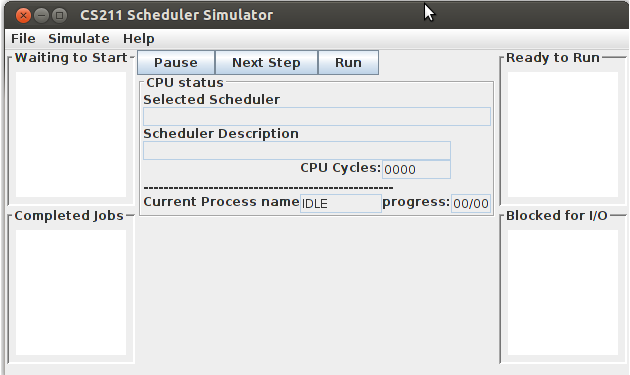
\epsfig{file=../testing/interface.png, height=5cm, width=9cm}
\caption{The interface for the scheduler simulator}
\end{figure}

\subsection{Jobs}
The jobs file were text files with the extension .jobs. These contained informa
tion on each process such as process name, priority, start time, cycles on cpu
and cycles blocked. These were used to test scheduling algorithms on the scheduler simulator.


\subsection{Shedulers}
The simulator came with one scheduler which was first come first serve. This acted as a base for the creating of the four other implemened schedulers. For each scheduler information on how it functions was gathered and then the first come first serve class was then modified. The first scheduler implemented was round robin, this was selected as it required the least modifications to the first come first serve class. This set the time to be two ticks and was tested with the test jobs files. The scheduler was then tweaked to confirm that it was working correctly.

The other three schedulers were implemented and tested using the first come first serve class as there base start point. The highest priority scheduler was designed and implemented to put jobs with highest priority to the front of the queue. The shortest time put jobs with the shortest time to completion at the head of the queue.

The final scheduler implemented was high response ratio next. This was designed to take into acound job length and how long the job had been waiting. Using these pieces of information new priorities could be calculated. The new priority was crated by adding wait time to time remaining and then dividing the answer by the remaining time. The largest of these calculated priorities go tothe head of the queue. 

\subsection{Class Diagrams}
Each scheduler class implements the scheduler interface. The interface has six methods defined. These are, getNextJob, addNewJob, returnJob, removeJob, reset and getJobList.

\subsection{First come first serve class}
This class implements the scheduler interface and uses all but the returnJob functions. This just passes the head of the queue back to be processed.

\subsection{Highest Priority Class}
This class implements the scheduler interface and makes use of all methods. The highest priority job is placed at the front on the cue when adding and removing.

\subsection{Shortest time first class}
This class implements the scheduler interface and uses all methods. This class will do the same as highest priority class but with the shortest length going to the head of the queue rather than the highest priority.

\subsection{Round robin}
This class implements the scheduler interface and uses all methods. This class allocates a time portion to each process at the head of the queue, when that time is used up it goes to the back of the queue.

\subsection{High response ration next}
This class implements the scheduler interface and uses all methods. This class takes into account the length of the job and the time it has been waiting in the queue. It then calculates the new priority and puts the job with the highest priority at the head od the queue.

\begin{figure}
\centering
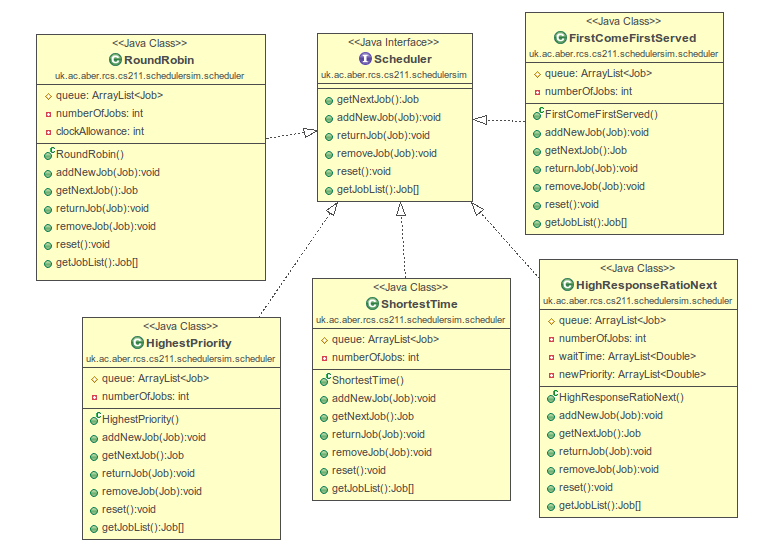
\epsfig{file=../design/class.png, height=5cm, width=9cm}
\caption{A class diagram of schedulers and their implemented interface}
\end{figure}



\section{Results}
Each scheduler was tested with five test jobs that were identical for each scheduelr.
\subsection{First Come First Serve Results}
The first scheduler tested was first come first serve and the results are as follows.

The first job to finish from the first test job file is CPU2 which was completed in thirteen cpu cycles. The job to finish first from test2 is CPU1 in twenty four cycles. The jobs that finished first from test3, test4 and test5 are CPU2 in fourty two cycles, CPU2 in thirteen cycles and CPU1 in fourty two cycles respectively. 

The mean time for this scheduler to finish a job is sixty two point eight cycles. This is third best at the mean time to finish a job and is expected as it is not ordering the jobs with any criteria in mind.

The mean overall processing time for all jobs using this scheduler comes to eighty seven cycles. This is fourth in this aspect compared to the other scheduling algorithms.

\subsection{Highest Priority Results}
The second scheduler tested is highest priority first. This takes the higher priority jobs and puts them at the head of the queue.

The numbers of cycles first job took to complete are as follows. For test, test2, test3, test4 and test5 the first job finished was IO1 in twenty seven cycles, CPU1 in twelve cycles, CPU2 in thirty one cycles, CPU1 in fourteen cycles and CPU1 in fourty two cycles respectively.

The mean time for the highest priority scheduler to finish a job is fifty eight point four cycles. This is second quickest at finishing jobs on average. The mean overall processing time for all jobs is eighty six point four.

\subsection{Highest Response Ratio Next Results}
The third scheduler tested is highest response ratio next which takes into account length of job and wait time.

The number of cycles first job took to complete are as follows. For test, test2, test3, test4 and test5 the first job finished was CPU2 in fourty cycles, CPU1 in fourty cycles, Inter in eighty one cycles, CPU2 in nineteen cycles and CPU1 in fourty three cycles respectively.

The mean time for high response ratio next scheduler to finish a job is sixty five cycles. This is fourth quickest at finishing jobs on average. The mean overall processing time for all jobs is eighty three point four cycles. This schedulers is second best at overall processing time on average.

\subsection{Round Robin Results}
The fourth scheduler, round robin, allocates a slice of time for each job to use. This allows even allocation of process power for each job.

The number of cycles first job took to complete are as follows. For test, test2
, test3, test4 and test5 the first job finished was CPU2 in fifty cycles, Inter in fourty three cycles, Inter in sixty eight cycles, CPU2 in twenty eight cycles and CPU3 in fifty one cycles respectively.

The mean time for round robin scheduler to finish a job is sixty seven point six cycles. This is the least effective at finishing a job quickly on average of the schedulers tested. The mean overall processing time for all jobs is eighty three point two. This is the best result of all the schedulers tested.

\subsection{Shortest Time Results}
This is the final scheduler tested and puts jobs in order of shortest time to complete at the head of the queue.

The number of cycles first job took to complete are as follows. For test, test2
, test3, test4 and test5 the first job finished was CPU1 in eleven cycles, CPU1 in eleven cycles, Inter in fifteen cycles, CPU1 in fourteen cycles and CPU3 in twenty one cycles respectively.

The mean time for shortest time scheduler to finish a job is fourty nine point eight cycles. This is the best at finishing a job quickly on average of schedulers tested. The mean overall processing time for all jobs is ninety two cycles. This is the worst out of all the schedulers tested.

\subsection{Overall Results}
On average the highest priority scheduler performed best meaning that of all the schedulers tested this was the one that worked well with regard to all aspects. The worst scheduler on average was shortest time scheduler despite being the fastest mean time per job.

The first come first serve had the least context switches overall. This is to be expected as there is no extra shuffling of the queue. Highest response ration next had the most context switches on average out of all the schedulers.

For full table of results see the testin.ods file in the testing folder.

\begin{figure}
\centering
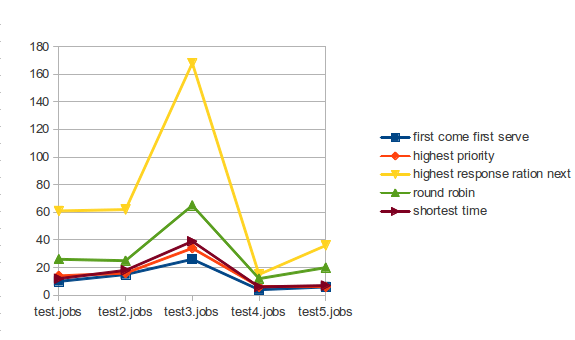
\epsfig{file=../testing/contexts.png, height=5cm, width=9cm}
\caption{A graph showing number of context switches for each scheduler}
\end{figure}

\begin{figure}
\centering
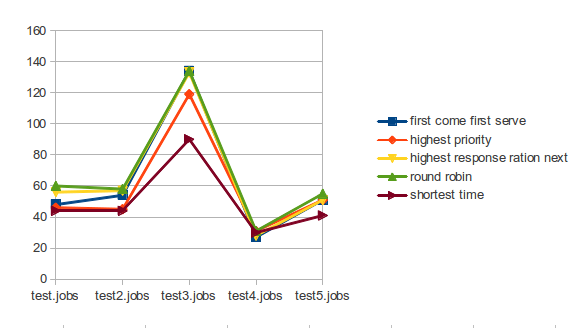
\epsfig{file=../testing/meanjob.png, height=5cm, width=9cm}
\caption{A graph showing mean time taken to complete a job for each scheduler}
\end{figure}

\begin{figure}
\centering
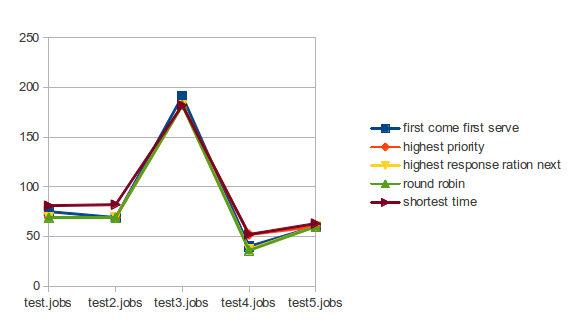
\epsfig{file=../testing/totalcpu.png, height=5cm, width=9cm}
\caption{A graph showing total cpu time for each scheduler}
\end{figure}

\section{Conclusions}
After testing these five schedulers it has shown that each scheduler has an advantage in different areas. To decide what scheduler is best to use you must first work out what it is going to be used for. Although highest priority proved itself to work consistantly well it may not always be the scheduler of choice.

The results for first come first serve and shortest time first were as expectedhowever, the highest response ration next scheduler result was interesting. I was expecting the mean elapsed duration to be shorter for this scheduler than what is shown in the results.

This could be developed further by looking into a wider range of scheduling algorithms and using some realistic data. With more testing it might be possible to combine or even develop a new and more effective scheduling algorithm.


\section{Executive Sumarry}
This report provides an analysis and evaluation of a few scheduling algorithms. These include first come first served, highest priority, shortest time, round robin and high response ratio next.

Methods of analysis include testing each scheduler against a series of varied sample jobs.

The finding show that highest priority performed the best andmost consistantly out of all the schedulers and that shortest time performed worst out of all the schedulers.

Conclusions are that highest priority is a good all round scheduler but a more specific scheduler might be needed for different tasks.

It is recommended that more schedulers are tested against a wider range of test jobs as this report only covers a few of the schedulers that exist.


% That's all folks!
\end{document}
